% ===========================================================================
% NotiBot — Pipeline de Datos para Noticias de Lima y Callao
% Presentación Beamer
% ===========================================================================
\documentclass[11pt,aspectratio=169,spanish]{beamer}

% ── Paquetes ────────────────────────────────────────────────────────────────
\usepackage[utf8]{inputenc}
\usepackage[T1]{fontenc}
\usepackage{babel}
\usepackage{graphicx}
\usepackage{booktabs}
\usepackage{xcolor}
\usepackage{hyperref}
\usepackage{listings}
\usepackage{tikz}
\usetikzlibrary{arrows.meta, positioning, shapes.geometric, fit, backgrounds}

% ── Tema ────────────────────────────────────────────────────────────────────
\usetheme{Madrid}
\usecolortheme{default}

% ── Colores personalizados ──────────────────────────────────────────────────
\definecolor{azul}{RGB}{30,27,75}        % Deep Indigo (brand)
\definecolor{verde}{RGB}{132,204,22}     % Lime (CTA)
\definecolor{celeste}{RGB}{14,165,233}   % Electric Blue (AI)
\definecolor{gris}{RGB}{100,100,100}

\setbeamercolor{structure}{fg=azul}
\setbeamercolor{title}{fg=white,bg=azul}
\setbeamercolor{frametitle}{fg=white,bg=azul}
\setbeamercolor{block title}{fg=white,bg=azul}
\setbeamercolor{block body}{fg=black,bg=azul!10}
\setbeamercolor{alerted text}{fg=verde}

% ── Código ──────────────────────────────────────────────────────────────────
\lstset{
  basicstyle=\ttfamily\small,
  keywordstyle=\color{azul},
  commentstyle=\color{gris},
  stringstyle=\color{verde},
  showstringspaces=false,
  breaklines=true,
  language=Python,
  aboveskip=2pt,
  belowskip=2pt,
}

% ── Metadatos ───────────────────────────────────────────────────────────────
\title[NotiBot — Pipeline de Datos]{
    NotiBot: Pipeline de Datos para Noticias\\
    de Lima y Callao
}
\subtitle{Recolección, Limpieza, Exploración, Procesamiento y División}
\author[]{NotiBot Team}
\date{\today}
\institute[]{Plataforma Inteligente de Noticias}

\begin{document}

% ===========================================================================
% PORTADA
% ===========================================================================
\begin{frame}[plain]
    \maketitle
\end{frame}

% ===========================================================================
% ÍNDICE
% ===========================================================================
\begin{frame}{Índice}
    \tableofcontents[hideallsubsections]
\end{frame}

% ===========================================================================
% SECCIÓN 1 — VISIÓN GENERAL
% ===========================================================================
\section{Visión General}
\subsection{Arquitectura del Pipeline}

\begin{frame}{Flujo General del Pipeline}
    \begin{center}
    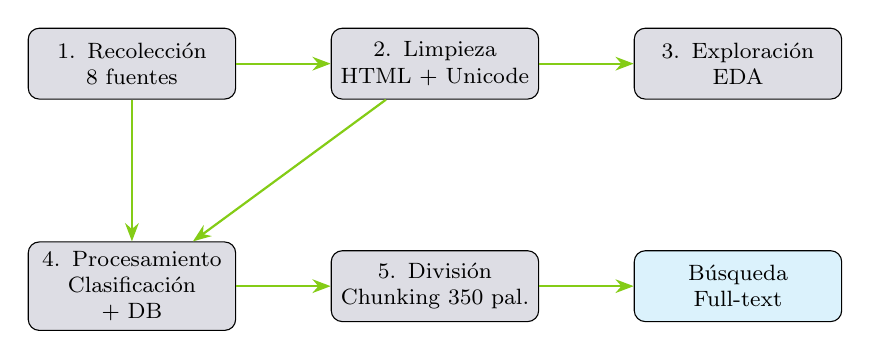
\begin{tikzpicture}[
        node distance=1.8cm and 1.2cm,
        block/.style={rectangle, draw, rounded corners, fill=azul!15, text width=2.4cm, align=center, minimum height=0.9cm, font=\footnotesize},
        arrow/.style={-{Stealth}, thick, verde}
    ]
        \node[block] (reco) {1. Recolección\\8 fuentes};
        \node[block, right=of reco] (limp) {2. Limpieza\\HTML + Unicode};
        \node[block, right=of limp] (expl) {3. Exploración\\EDA};
        \node[block, below=of reco] (proc) {4. Procesamiento\\Clasificación + DB};
        \node[block, right=of proc] (div) {5. División\\Chunking 350 pal.};

        \draw[arrow] (reco) -- (limp);
        \draw[arrow] (limp) -- (expl);
        \draw[arrow] (reco) -- (proc);
        \draw[arrow] (limp) -- (proc);
        \draw[arrow] (proc) -- (div);

        \node[block, right=of div, fill=celeste!15] (busq) {Búsqueda\\Full-text};
        \draw[arrow] (div) -- (busq);
    \end{tikzpicture}
    \end{center}

    \vspace{0.5cm}
    \begin{block}{Stack tecnológico}
        \begin{itemize}
            \item \textbf{Backend:} Python 3.14, FastAPI, SQLAlchemy async, asyncpg
            \item \textbf{Base de datos:} PostgreSQL 16, índices GIN, tsvector
            \item \textbf{EDA:} pandas, matplotlib, seaborn, nltk, wordcloud
            \item \textbf{Frontend:} Angular 21, SCSS
        \end{itemize}
    \end{block}
\end{frame}

% ===========================================================================
% SECCIÓN 2 — RECOLECCIÓN DE DATOS
% ===========================================================================
\section{Recolección de Datos}

\begin{frame}{Fuentes de Noticias}
    \begin{table}[h]
    \centering
    \small
    \begin{tabular}{clll}
        \toprule
        \textbf{ID} & \textbf{Periódico} & \textbf{Método} & \textbf{Tipo} \\
        \midrule
        1 & La República & Sitemap XML & Sitemap único \\
        2 & El Comercio & Sitemaps por sección & 9 secciones \\
        3 & Peru21 & HTML sections & 10 secciones \\
        4 & Diario Correo & RSS Arc XP & 6 secciones \\
        5 & Gestión & RSS Arc XP & 6 secciones \\
        6 & Trome & RSS Arc XP & 5 secciones \\
        7 & Ojo & RSS Arc XP & 7 secciones \\
        8 & La Razón & Sitemap WordPress & Yoast SEO \\
        \bottomrule
    \end{tabular}
    \end{table}

    \begin{alertblock}{Nota}
        Las 8 fuentes se ejecutan en modo \texttt{--daily}, iterando día a día.
        El modo \texttt{--today} procesa solo el día actual.
    \end{alertblock}
\end{frame}

\begin{frame}{Métodos de Recolección}
    \begin{columns}[T]
        \begin{column}{0.48\textwidth}
            \textbf{Sitemaps XML (3 fuentes)}
            \begin{itemize}
                \item Parseo de \texttt{<url><loc>} y \texttt{<lastmod>}
                \item Filtrado por rango de fechas
                \item Extracción de artículo vía HTTP GET + BeautifulSoup
                \item Metadatos: JSON-LD, Open Graph, meta tags
                \item ThreadPoolExecutor para concurrencia
            \end{itemize}
        \end{column}
        \begin{column}{0.48\textwidth}
            \textbf{RSS Arc XP (4 fuentes)}
            \begin{itemize}
                \item Feed URL: \texttt{\{base\}/arcio/rss/category/\{sec\}/}
                \item \texttt{<content:encoded>} incluye HTML completo
                \item \textbf{No requiere scrapeo por artículo}
                \item $\sim$6 HTTP requests por fuente por día
                \item Extracción directa desde el XML del feed
            \end{itemize}
        \end{column}
    \end{columns}

    \vspace{0.5cm}
    \begin{columns}[T]
        \begin{column}{0.48\textwidth}
            \textbf{HTML Sections (1 fuente)}
            \begin{itemize}
                \item Peru21: sitemap roto (lastmod 2012)
                \item Scrapeo de páginas de sección \\
                  (\texttt{/lima/}, \texttt{/politica/}, etc.)
                \item Extracción desde \texttt{article.node--type-article}
                \item Fechas confiables desde \texttt{<time datetime>}
            \end{itemize}
        \end{column}
        \begin{column}{0.48\textwidth}
            \textbf{WordPress Sitemap (1 fuente)}
            \begin{itemize}
                \item La Razón: sitemap WordPress + Yoast SEO
                \item Filtrado de post-sitemaps
                \item \texttt{articleSection} puede ser array
                \item Ventana de 30 días para reducir carga
            \end{itemize}
        \end{column}
    \end{columns}
\end{frame}

\begin{frame}{Arquitectura de Requests}
    \begin{block}{Sesión HTTP compartida}
        \begin{itemize}
            \item \texttt{requests.Session} única para todas las fuentes
            \item User-Agent: Chrome 124 en Windows
            \item Accept-Language: \texttt{es-PE,es;q=0.9}
            \item Estrategia de retry: 3 reintentos con backoff 1s
            \item Pool de conexiones: 10 pool / 20 max
        \end{itemize}
    \end{block}

    \vspace{0.3cm}
    \begin{block}{Concurrencia}
        \begin{itemize}
            \item \texttt{ThreadPoolExecutor} con 5 workers (configurable)
            \item La República: extracción paralela de artículos
            \item El Comercio y La Razón: ThreadPoolExecutor para artículos
            \item Arc XP RSS: procesamiento secuencial (no se necesita por artículo)
        \end{itemize}
    \end{block}
\end{frame}

\begin{frame}[fragile]{Metadatos Extraídos}
    Campos comunes extraídos de cada artículo:

    \begin{columns}[T]
        \begin{column}{0.5\textwidth}
            \begin{itemize}
                \item \texttt{url}, \texttt{url\_canonica}, \texttt{url\_imagen}
                \item \texttt{titulo}, \texttt{subtitulo}
                \item \texttt{autor}
                \item \texttt{seccion\_fuente}
            \end{itemize}
        \end{column}
        \begin{column}{0.5\textwidth}
            \begin{itemize}
                \item \texttt{fecha\_publicacion}
                \item \texttt{fecha\_actualizacion}
                \item \texttt{contenido\_limpio} (texto plano)
                \item \texttt{contenido\_html} (HTML original)
                \item \texttt{contenido\_crudo} (respuesta raw)
                \item \texttt{keywords}
            \end{itemize}
        \end{column}
    \end{columns}

    \vspace{0.3cm}
    \begin{block}{Fuentes de metadatos (en orden de prioridad)}
        \begin{enumerate}
            \item JSON-LD (\texttt{NewsArticle}, \texttt{ReportageNewsArticle})
            \item Open Graph / meta tags (\texttt{og:title}, \texttt{article:published\_time})
            \item Heurísticas HTML (h1, selectores CSS específicos por fuente)
        \end{enumerate}
    \end{block}
\end{frame}

% ===========================================================================
% SECCIÓN 3 — LIMPIEZA DE DATOS
% ===========================================================================
\section{Limpieza de Datos}

\begin{frame}[fragile]{Normalización de Texto}
    \begin{block}{Función \texttt{normalize\_text()}}
        \begin{enumerate}
            \item Conversión a minúsculas
            \item Normalización Unicode NFKD:
            \texttt{unicodedata.normalize("NFD", text)}
            \item Eliminación de caracteres combinantes (categoría \texttt{Mn})
            $\rightarrow$ quita tildes: \textit{``acción''} $\to$ \textit{``accion''}
        \end{enumerate}
    \end{block}

    \vspace{0.3cm}
    \begin{alertblock}{Importante}
        La normalización \textbf{solo} se usa para matching geográfico.
        El texto original con tildes se preserva íntegramente en la base de datos.
    \end{alertblock}
\end{frame}

\begin{frame}{Limpieza HTML por Fuente}
    \begin{table}[h]
    \small
    \begin{tabular}{lp{8cm}}
        \toprule
        \textbf{Fuente} & \textbf{Método de limpieza} \\
        \midrule
        La República & \texttt{get\_text()} sobre divs de contenido, join con espacio \\
        El Comercio  & \texttt{get\_text()} sobre \texttt{p.sc\_\_font-paragraph} \\
        Peru21       & Descomposición de \texttt{div.publicidad-*}, \texttt{div.embedded-entity}, \texttt{section} antes de extraer \\
        Arc XP RSS   & Descomposición de \texttt{script, style, div.publicidad}, luego \texttt{get\_text()} \\
        La Razón     & Descomposición de \texttt{div.code-block}, \texttt{script, style, ins, iframe} \\
        \bottomrule
    \end{tabular}
    \end{table}

    \begin{block}{Resultado}
        \begin{itemize}
            \item \texttt{contenido\_limpio}: texto plano, HTML tags eliminados, whitespace colapsado
            \item \texttt{contenido\_html}: HTML original preservado
            \item \texttt{contenido\_crudo}: respuesta HTTP sin procesar
        \end{itemize}
    \end{block}
\end{frame}

\begin{frame}[fragile]{Limpieza EDA (NLP)}
    \begin{block}{Función \texttt{limpiar\_texto()} en \texttt{eda\_nlp.py}}
        \begin{itemize}
            \item Conversión a minúsculas
            \item Eliminación de URLs: \texttt{http\textbackslash S+|www\textbackslash S+}
            \item Conservación de caracteres alfabéticos españoles: \texttt{a-záéíóúñ}
            \item Colapso de whitespace múltiple
        \end{itemize}
    \end{block}

    \vspace{0.3cm}
    \begin{block}{Stopwords personalizadas}
        NLTK Spanish stopwords + adiciones específicas del dominio:
        \begin{itemize}
            \item \textit{noticias, noticia, lima, callao, perú, peru}
            \item \textit{comercio, república, republica, día}
            \item Más palabras funcionales comunes en español
        \end{itemize}
    \end{block}
\end{frame}

% ===========================================================================
% SECCIÓN 4 — EXPLORACIÓN DE DATOS
% ===========================================================================
\section{Exploración de Datos}

\begin{frame}{Scripts EDA}
    \begin{table}[h]
    \small
    \begin{tabular}{lll}
        \toprule
        \textbf{Script} & \textbf{Enfoque} & \textbf{Salida} \\
        \midrule
        \texttt{eda\_01} & Características generales & Consola \\
        \texttt{eda\_02} & Distribuciones & \texttt{eda\_distribuciones.png} \\
        \texttt{eda\_03} & Longitudes de texto & \texttt{eda\_longitudes.png} \\
        \texttt{eda\_04} & Frecuencia de palabras & \texttt{eda\_frecuencia\_palabras.png} \\
        \texttt{eda\_05} & Wordclouds & \texttt{wordclouds\_eda.png} \\
        \bottomrule
    \end{tabular}
    \end{table}

    \begin{block}{Exportación desde PostgreSQL}
        \begin{itemize}
            \item \texttt{export\_from\_db.py}: SQLAlchemy síncrono con psycopg2
            \item JOIN \texttt{noticias} $\bowtie$ \texttt{noticias\_contenido}
            \item Salida JSON con preview de contenido (500 caracteres)
        \end{itemize}
    \end{block}
\end{frame}

\begin{frame}{Distribuciones}
    \begin{center}
        \includegraphics[width=0.9\textwidth,height=0.78\textheight,keepaspectratio]%
            {img/eda_distribuciones.png}
    \end{center}
\end{frame}

\begin{frame}{Longitudes}
    \begin{center}
        \includegraphics[width=0.9\textwidth,height=0.78\textheight,keepaspectratio]%
            {img/eda_longitudes.png}
    \end{center}
\end{frame}

\begin{frame}{Frecuencia de Palabras}
    \begin{center}
        \includegraphics[width=\textwidth,height=0.8\textheight,keepaspectratio]%
            {img/eda_frecuencia_palabras.png}
    \end{center}
\end{frame}

\begin{frame}{Wordclouds}
    \begin{center}
        \includegraphics[width=0.85\textwidth,height=0.78\textheight,keepaspectratio]%
            {img/wordclouds_eda.png}
    \end{center}
\end{frame}

% ===========================================================================
% SECCIÓN 5 — PROCESAMIENTO DE DATOS
% ===========================================================================
\section{Procesamiento de Datos}

\begin{frame}{Clasificación Geográfica}
    \begin{columns}[T]
        \begin{column}{0.55\textwidth}
            \textbf{Algoritmo de 3 pasadas}
            \begin{enumerate}
                \item \textbf{Distritos} — Regex con \texttt{\textbackslash b} word boundaries contra 43 distritos de Lima + 7 del Callao
                \item \textbf{Keywords Lima} — 33 términos (\textit{lima, miraflores, surco, comas...})
                \item \textbf{Keywords Callao} — 8 términos (\textit{callao, chalaco, ventanilla...})
            \end{enumerate}
        \end{column}
        \begin{column}{0.45\textwidth}
            \begin{block}{Resultado}
                \begin{itemize}
                    \item \texttt{scope\_geografico}: \\
                      \textit{lima\_metropolitana} | \textit{callao}
                    \item \texttt{provincia}: Lima | Callao
                    \item \texttt{distrito}: nombre del distrito
                    \item \texttt{ubigeo}: código INEI
                \end{itemize}
            \end{block}
        \end{column}
    \end{columns}

    \begin{alertblock}{Filtrado estricto}
        Artículos sin coincidencia geográfica ($\approx$ \texttt{desconocido}) son \textbf{descartados}.
        Solo se almacenan noticias relevantes para Lima Metropolitana y Callao.
    \end{alertblock}
\end{frame}

\begin{frame}{Inferencia de Categoría}
    \begin{columns}[T]
        \begin{column}{0.5\textwidth}
            \textbf{14 categorías normalizadas}
            \begin{itemize}
                \item Política
                \item Sociedad
                \item Nacional
                \item Deportes
                \item Economía
                \item Mundo
                \item Espectáculos
                \item Cultura
                \item Tecnología
                \item Opinión
                \item Tendencia
                \item Ciencia
                \item Datos
                \item Historia
            \end{itemize}
        \end{column}
        \begin{column}{0.5\textwidth}
            \textbf{Método}
            \begin{enumerate}
                \item Matching por subcadena contra slugs de sección
                \item Fallback: keywords en el título (gol, inflación, elecciones...)
                \item Último recurso: nombre de sección en formato título
            \end{enumerate}
            \vspace{0.3cm}
            \begin{block}{Ejemplo}
                \texttt{"politica-nacional"} $\to$ \textbf{Política}\\
                \texttt{"deporte-total"} $\to$ \textbf{Deportes}\\
                \texttt{"g-de-gestion"} $\to$ \textbf{Economía}
            \end{block}
        \end{column}
    \end{columns}
\end{frame}

\begin{frame}{Escritura a Base de Datos}
    \begin{block}{Arquitectura de escritura}
        \begin{itemize}
            \item Clase \texttt{NewsDBWriter}: SQL crudo vía \texttt{sqlalchemy.text()}
            \item \textbf{Sin ORM} — performance y control sobre las queries
            \item Sesión asíncrona con \texttt{async\_sessionmaker}
            \item \texttt{engine.dispose()} obligatorio tras cada escritura
        \end{itemize}
    \end{block}

    \vspace{0.3cm}
    \begin{table}[h]
    \small
    \begin{tabular}{ll}
        \toprule
        \textbf{Tabla} & \textbf{Dedup / Conflicto} \\
        \midrule
        \texttt{fuentes} & \texttt{ON CONFLICT (slug) DO UPDATE} \\
        \texttt{fuentes\_seeds} & Verificación previa por (id\_fuente, url\_seed) \\
        \texttt{noticias} & \texttt{ON CONFLICT (url\_original) DO UPDATE} \\
        \texttt{noticias\_contenido} & \texttt{ON CONFLICT (id\_noticia) DO UPDATE} \\
        \texttt{scraping\_logs} & Sin conflicto (logs append-only) \\
        \texttt{pipeline\_jobs} & Insert via ORM (chunking auto-trigger) \\
        \bottomrule
    \end{tabular}
    \end{table}
\end{frame}

\begin{frame}[fragile]{Hashes y Deduplicación}
    \begin{block}{Cálculo de hashes}
        \begin{itemize}
            \item \texttt{hash\_titulo}: SHA-256 del título $\to$ 32 hex chars
            \item \texttt{hash\_contenido}: SHA-256 del contenido $\to$ 32 hex chars
            \item Calculados inline antes del INSERT
        \end{itemize}
    \end{block}

    \vspace{0.3cm}
    \begin{alertblock}{Estrategia real de deduplicación}
        \begin{itemize}
            \item \textbf{Clave primaria:} \texttt{ON CONFLICT (url\_original)}
            \item Los hashes se almacenan pero \textbf{no se usan} para detectar duplicados
            \item Si la URL ya existe, se actualizan título, subtítulo, autor, imagen y hash
        \end{itemize}
    \end{alertblock}
\end{frame}

% ===========================================================================
% SECCIÓN 6 — DIVISIÓN DE DATOS
% ===========================================================================
\section{División de Datos}

\begin{frame}[fragile]{Chunking — Estrategia}
    \begin{block}{Algoritmo \texttt{split\_text\_into\_chunks()}}
        \begin{enumerate}
            \item \textbf{Split por párrafos}: \texttt{re.split(r"\textbackslash n\textbackslash s*\textbackslash n", text)}
            \item \textbf{Acumulación}: agrega párrafos hasta alcanzar \textbf{350 palabras}
            \item \textbf{Párrafos largos}: split adicional por oraciones \\
              \texttt{re.split(r"(?<=[.!?])\textbackslash s+", paragraph)}
            \item \textbf{Join}: chunks unidos con doble salto de línea
        \end{enumerate}
    \end{block}

    \vspace{0.3cm}
    \begin{columns}[T]
        \begin{column}{0.5\textwidth}
            \textbf{Metadatos por chunk}
            \begin{itemize}
                \item \texttt{chunk\_index}: posición
                \item \texttt{texto\_chunk}: contenido
                \item \texttt{tokens\_estimados}:\\
                  $\text{palabras} \times 1.3$
                \item \texttt{inicio\_char} / \texttt{fin\_char}
            \end{itemize}
        \end{column}
        \begin{column}{0.5\textwidth}
            \textbf{Texto completo}
            \begin{itemize}
                \item Título + \texttt{"\textbackslash n\textbackslash n"} + contenido
                \item Cada chunk incluye contexto del título
            \end{itemize}
        \end{column}
    \end{columns}
\end{frame}

\begin{frame}[fragile]{Pipeline de Dos Pasos}
    \begin{block}{Paso 1: Chunking}
        \begin{enumerate}
            \item Carga \texttt{NoticiaContenido.contenido\_limpio} + \texttt{Noticia.titulo}
            \item Concatena título + contenido
            \item Ejecuta \texttt{split\_text\_into\_chunks()}
            \item Inserta en \texttt{noticias\_chunks} con \texttt{ON CONFLICT DO NOTHING}
            \item Crea job de vectorización
        \end{enumerate}
    \end{block}

    \vspace{0.3cm}
    \begin{block}{Paso 2: Vectorización (tsvector)}
        \begin{itemize}
            \item \texttt{to\_tsvector('spanish', titulo)} $\to$ peso \textbf{A}
            \item \texttt{to\_tsvector('spanish', subtitulo)} $\to$ peso \textbf{B}
            \item \texttt{to\_tsvector('spanish', contenido)} $\to$ peso \textbf{C}
            \item Inserta/actualiza en \texttt{noticias\_busqueda}
        \end{itemize}
    \end{block}
\end{frame}

\begin{frame}[fragile]{Búsqueda Full-Text con PostgreSQL}
    \begin{block}{Índice GIN + tsvector}
        \begin{itemize}
            \item Configuración de búsqueda: \texttt{'spanish'} (diccionario español incorporado)
            \item \texttt{setweight()} asigna jerarquía de relevancia: \\
              Título (A) > Subtítulo (B) > Contenido (C)
            \item Índice GIN sobre la columna \texttt{documento\_tsv}
        \end{itemize}
    \end{block}

    \vspace{0.3cm}
    \begin{block}{Procesamiento de jobs}
        \begin{itemize}
            \item \texttt{process\_pending\_jobs()}: procesa hasta 20 jobs por llamada
            \item Orden: prioridad $\to$ created\_at
            \item Jobs fallidos: \texttt{estado="error"}, traceback almacenado
            \item Reintentos: contador \texttt{intentos} incrementado
        \end{itemize}
    \end{block}
\end{frame}

% ===========================================================================
% SECCIÓN 7 — RESUMEN
% ===========================================================================
\section{Resumen}

\begin{frame}{Pipeline Completo}
    \begin{center}
    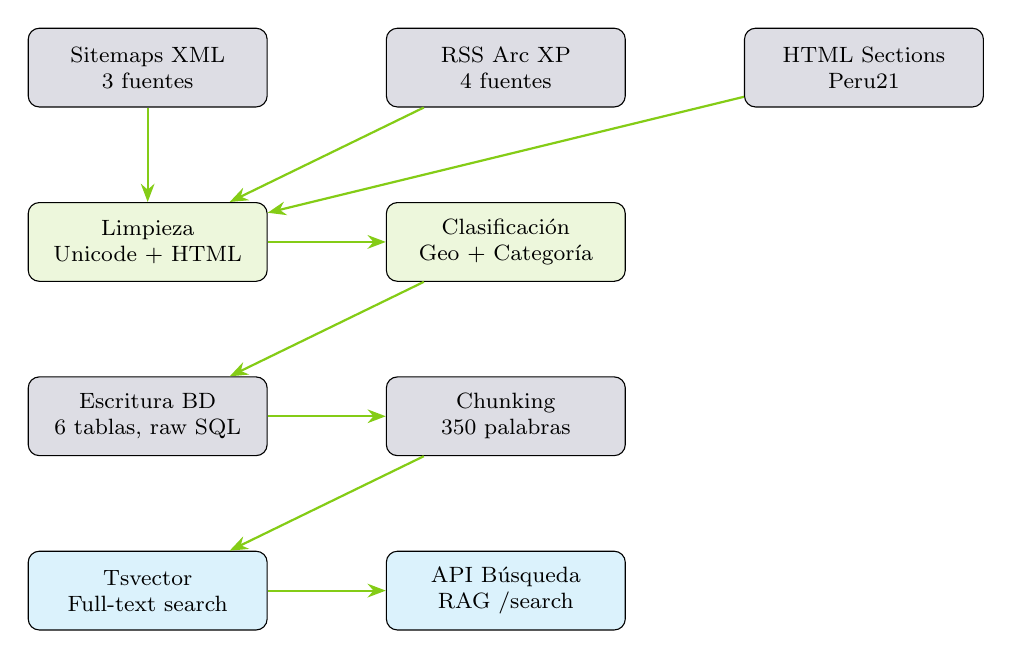
\begin{tikzpicture}[
        node distance=1.8cm and 1.5cm,
        block/.style={rectangle, draw, rounded corners, fill=azul!15, text width=2.8cm, align=center, minimum height=1cm, font=\footnotesize},
        arrow/.style={-{Stealth}, thick, verde},
        label/.style={font=\footnotesize\color{gris}}
    ]
        \node[block] (sitemap) {Sitemaps XML\\3 fuentes};
        \node[block, right=of sitemap] (rss) {RSS Arc XP\\4 fuentes};
        \node[block, right=of rss] (html) {HTML Sections\\Peru21};

        \node[block, below=1.2cm of sitemap, fill=verde!15] (clean) {Limpieza\\Unicode + HTML};
        \node[block, right=of clean, fill=verde!15] (class) {Clasificación\\Geo + Categoría};

        \node[block, below=1.2cm of clean] (db) {Escritura BD\\6 tablas, raw SQL};
        \node[block, right=of db] (chunk) {Chunking\\350 palabras};

        \node[block, below=1.2cm of db, fill=celeste!15] (tsv) {Tsvector\\Full-text search};
        \node[block, right=of tsv, fill=celeste!15] (search) {API Búsqueda\\RAG /search};

        \draw[arrow] (sitemap) -- (clean);
        \draw[arrow] (rss) -- (clean);
        \draw[arrow] (html) -- (clean);
        \draw[arrow] (clean) -- (class);
        \draw[arrow] (class) -- (db);
        \draw[arrow] (db) -- (chunk);
        \draw[arrow] (chunk) -- (tsv);
        \draw[arrow] (tsv) -- (search);
    \end{tikzpicture}
    \end{center}

    \vspace{0.3cm}
    \begin{block}{Cifras clave}
        \begin{itemize}
            \item 8 fuentes activas de periódicos peruanos
            \item 50 distritos cubiertos (43 Lima + 7 Callao)
            \item 14 categorías normalizadas
            \item $\sim$455 tokens por chunk (350 palabras $\times$ 1.3)
            \item Búsqueda full-text con ranking ponderado (A $>$ B $>$ C)
        \end{itemize}
    \end{block}
\end{frame}

% ===========================================================================
% CIERRE
% ===========================================================================
\begin{frame}[plain]
    \begin{center}
        \Huge\textcolor{azul}{¿Preguntas?}

        \vspace{1cm}
        \normalsize
        NotiBot — Plataforma Inteligente de Noticias\\
        Lima y Callao
    \end{center}
\end{frame}

\end{document}
